\section{Grundlagen}
In diesem Kapitel werden die benötigten Konzepte und Algorithmen erklärt, die für das Verständnis der Arbeit notwendig sind.
In \cref{sec:entscheidungsbaum} wird auf die grundlegende Funktionsweise von Entscheidungsbaum-Algorithmen, in speziellem den CART-Algorithmus, eingegangen.
Daraufhin wird in \cref{sec:randomforest} das Vorgehen von Random-Forest-Algorithmen beschrieben. In \cref{sec:prolog}
wird die Programmiersprache Prolog kurz eingeführt.


\subsection{Entscheidungsbaum} \label{sec:entscheidungsbaum}
Entscheidungsbaumalgorithmen sind sogenannte nicht-parametrische Methoden, das heißt, dass vor der
Entstehung des Baums keine Parameter vorgegeben werden müssen und die Struktur des Baums von den Daten abhängt.
Ein Entscheidungsbaum ist eine hierarchische Struktur die aus internen Entscheidungsknoten und terminalen Blättern besteht.
Jeder Entscheidungsknoten beinhaltet eine einfache Funktion mit diskreten Ergebnissen, die die Zweige repräsentieren.
Diese Funktionen werden so gewählt, dass sie den Eingaberaum in immer kleinere Regionen unterteilen, welche wiederum
unterteilt werden, je weiter man den Pfad von der Wurzel nach unten folgt.
Ein terminales Blatt entsteht dann, wenn die lokale Region im Eingaberaum nicht weiter unterteilt werden soll.
Im Falle von Klassifikationsbäumen ist das meist der Fall, wenn die Region nur aus den gleichen diskreten Werten besteht,
während es bei Regressionsbäumen sehr ähnliche stetige Werte sind.
Ein beispielhafter Entscheidungsbaum und die dazugehörige Unterteilung des Eingaberaums ist in \cref{fig:baum}~\cite{Alpaydin+2022} dargestellt.
\begin{figure}[h]
  \centering
  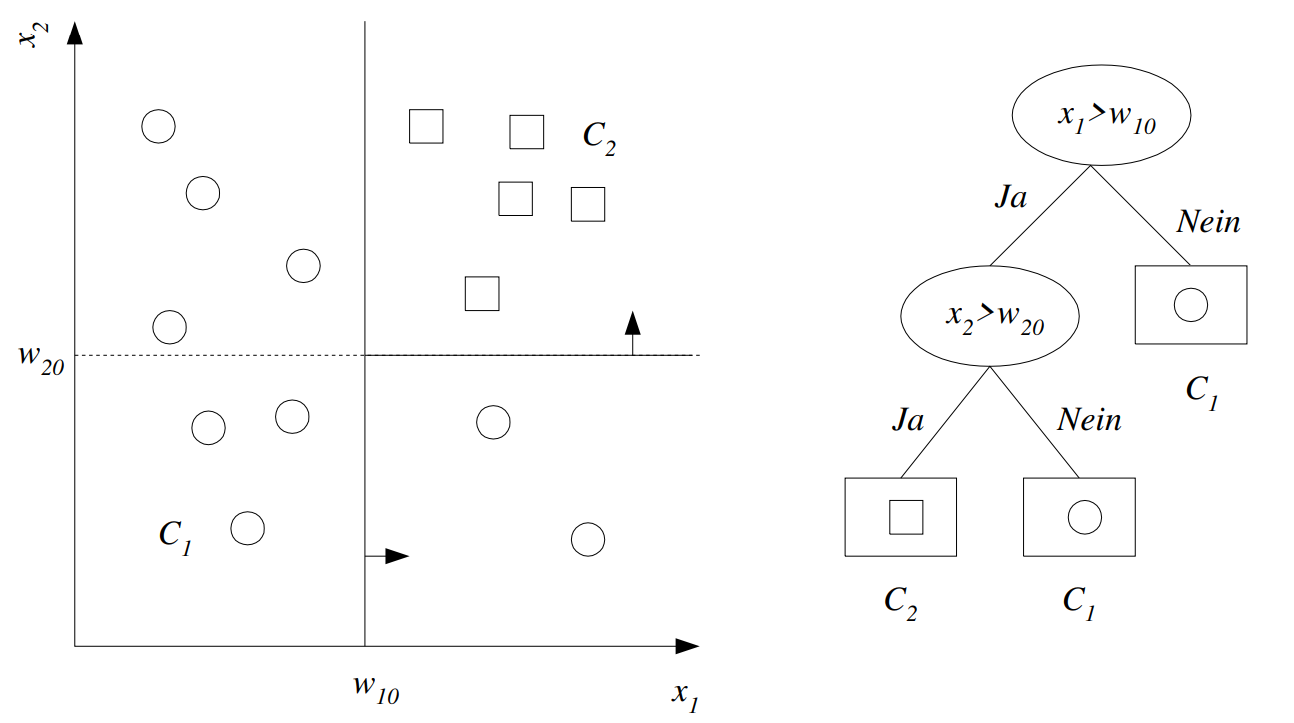
\includegraphics[width=10cm]{fig/baum.png}
  \caption{beispielhafter Entscheidungsbaum und Unterteilung. Ovale sind Entscheidungsknoten, Vierecke sind Blattknoten.}%
  \label{fig:baum}
\end{figure}
Bei gegebener Eingabe wird nun an jedem Knoten das Ergebnis der entsprechenden Funktion berechnet. In Abhängigkeit von dem Ergbnis
wird daraufhin der Zweig ausgewählt, welcher entlang gegangen wird. Das wird so lange wiederhohlt, bis man an in einem
Blattknoten angekommen ist. Der in diesem Blatt stehende Wert wird dann als Ausgabe benutzt.

In dieser Arbeit geht es um den CART Algorithmus, deswegen wird im Folgenden
nur die typische Vorgehensweise~\cite{CRAWFORD1989197} für diesen Algorithmus vorgestellt.
Diese ist in \cref{alg:baum} exemplarisch dargestellt.
\begin{algorithm}
  \caption{Training eines Entscheidungsbaums}%
  \label{alg:baum}
  \begin{algorithmic}[1]
    \Function{CreateTree}{Data}
      \If{\Call{Abbruchbedingung}{D} \(=\) true}
        \State label \(\gets\) \Call{Klasse}{D}
        \State \Return label
      \EndIf
      \State bestValue \(\gets \infty\)
      \State \(\mathit{bestSplit} \gets \) NIL
      \State splits \(\gets\) \Call{erstelleSplitliste}{D}
      \ForAll{\(s \in splits\)}
        \State \(\mathit{value} \gets \) \Call{KombiniertGini}{D, s}
        \If{\(\mathit{value} < \mathit{bestValue}\)}
          \Comment{Aktualisiere besten Wert}
          \State \(\mathit{bestValue} \gets \mathit{value}\)
          \State \(\mathit{bestSplit} \gets s\)
        \EndIf
      \EndFor
      \State leftTree, rightTree \(\gets\) \Call{aufteilen}{D,bestSplit}
      \State leftRes \(\gets\) \Call{CreateTree}{leftTree}
      \State rightRes \(\gets\) \Call{CreateTree}{rightTree}
      \State \Return \((s, leftRes, rightRes)\)
    \EndFunction
  \end{algorithmic}
\end{algorithm}
Der Baum besteht ursprünglich nur aus einen Wurzelknoten und beinhaltet den gesamten Datensatz T.
Als erstes wird die Menge aller möglichen binären Aufteilungen, von T, durchsucht, bis eine optimale
gefunden wurde. Was eine optimale Aufteilung ist, wird dabei durch ein Maß der Unreinheit bestimmt, welches minimiert
werden muss. Typischerweise benutzt der CART Algorithmus den Gini-Index für Klassifikation, abgebildet in \cref{eq:gini}.
Im Falle der Regression wird meist die Residuenquadratsumme benutzt, abgebildet in \cref{eq:rss}.
\begin{align}
    Gini(T)       & = 1 - \sum_{i=1}^n p_i^2 \label{eq:gini} \\
    \mathit{RSS}(T)       & = \sum_{i=1}^n (\bar{y} - x_i)^2 \label{eq:rss} 
  \end{align}
Hier ist \(p_i\) die relative Häufigkeit von der i-ten Klasse in T, während \(\bar{y}\) das arithmetische Mittel der Zielvariablen
in T ist und \(x_i\) die Zielvariable des i-ten Datenpunkts in T.
Diese Maße werden benutzt um die Reinheit eines einzelnen Knoten zu messen.
Um eine optimale Aufteilung zu finden, zum Beispiel, im Fall der Klassifikation mit Gini-Unreinheit,
muss \cref{eq:combgini} minimiert werden.
\begin{align}
    Gini(T)_{Split}       & = N_1/N * Gini(T_1) + N_2/N * Gini(T_2) \label{eq:combgini}
  \end{align}
Hier ist der Datensatz T in zwei Teile, \(T_1\) und \(T_2\), aufgeteilt und \(N_1\) und \(N_2\) geben die Anzahl an Datenpunkten
in der jeweiligen Teilmenge an.
Eine Aufteilung durch stetige Attribute nimmt dabei eine Regel der Form,
 \(A \leq r\) 
an, wobei r die Mitte von zwei beliebigen, unterschiedlichen Datenpunkten ist. Für ein kategorisches Attribut, welches die Werte
\(D_1\) bis \(D_n\) annehmen kann, nimmt die Aufteilung die Form \(A \in D_T\) an, wobei \(D_T\) eine Teilmenge von \{\(D_1\),...,\(D_n\)\} ist.
Nachdem eine optimale Aufteilung gefunden wurde, werden zwei Nachfolgerknoten, für den Wurzelknoten, erstellt.
Der linke enthält die Datenpunkte aus dem Datensatz, die die Regeln erfüllen, während der rechte den restlichen
Datensatz enthält.
Dieser Prozess nun wird rekursiv auf jedes Blatt angewendet, bis eine Abbruchbedingung erreicht ist. Eine Abbruchbedingung
kann einsetzen, wenn der Datensatz in einem Blatt zu klein ist, nur noch eine Klasse in allen Datenpunkten vertreten ist oder
sich die Datenpunkte nicht mehr unterscheiden lassen.
Da ein Entscheidungsbaum in den meisten Fällen unter \enquote{overfitting} leidet, wird dieser am Ende gestutzt.
Das Pruning ist ein komplexer Vorgang, der nicht in meiner Implementierung angewandt wurde, deswegen wird hier nicht näher
darauf eingegangen.

\subsection{Random Forest} \label{sec:randomforest}
Nach Breiman ist ein Random Forest \cite{Breiman2001} ein Klassifikator der aus einer Sammlung von
baumartigen Klassifikatoren besteht, welche aus unabhängig identisch verteilten Zufallsvektoren erstellt wurden,
und jeder Baum stimmt für die beliebteste Klasse der Eingabe.
Random Forest gehört zu den sogenannten \enquote{Ensemble Methoden}. Der Gedanke hinter diesen Methoden ist es,
das Problem der Instabilität von Entscheidungsbäumen zu lösen~\cite{Strobl2009-hw}, indem, bei Vorhersagen, der Durchschnitt von mehreren Bäumen genommen
wird. Durch diese Technik soll auch das Problem gelöst werden, dass Entscheidungsbäume sehr empfindlich gegenüber Änderungen
im Trainingsdatensatz reagieren.

Ein Random-Forest-Algorithmus besteht aus zwei Hauptbestandteilen: Bagging~\cite{breiman1996bagging} und
Feature Randomness.
Bagging (\enquote{bootstrap aggregating}) ist ein Verfahren das 1996 von Breiman vorgestellt wurde um
die Präzision von instabilen Verfahren, wie Entscheidungsbäumen, zu verbessern.
Beim bagging werden aus einem N großen Datensatz, N zufällige Instanzen mit zurücklegen gezogen.
Diese N Instanzen werden dann als Datensatz benutzt um einen Klassifikator zu trainieren. Dieser Vorgang
wird mehrfach wiederholt, bis man genug Klassifikatoren trainiert hat.
Um eine Vorhersage zu treffen, wird eine Vorhersage von allen Klassifikatoren getroffen. Anschließend
wird für die finale Vorhersage ein Mehrheitsentscheid getroffen, wobei alle Klassifikatoren eine Stimme haben.
Bei einem Random Forest sind diese Klassifikatioren Entscheidungsbäume.

Jedoch werden die Klassifikatoren nicht nur mit einem zufällig erzeugten Datensatz trainiert.
Bei dem Training von Entscheidungsbäumen in einem Random Forest wird zudem Feature Randomness eingesetzt.
Das heißt, dass bei der Konstruktion nicht alle Attribute der Instanzen im Datensatz genutzt werden.
Stattdessen wird voher eine zufällige Teilmenge aller Attribute erstellt, die während des Trainings benutzt werden.
Wie groß die Teilmenge ist, hängt davon ab, ob ein Klassifikationsbaum oder Regressionsbaum trainiert wird.
In \enquote{The Elements of Statistical Learning: Data Mining, Inference, and Prediction} wird vorgeschlagen,
dass man im Falle der Klassifikation \cref{eq:att-klass} und der Regression \cref{eq:att-reg} benutzt.
Hier ist m die Anzahl der Attribute, die eine Instanz besitzt.
\begin{align}
    M_{Klassifikation}       & = \lfloor\sqrt{m}\rfloor \label{eq:att-klass} \\
    M_{Regression}       & = \lfloor{m/3}\rfloor \label{eq:att-reg}
  \end{align}
Somit wird in einem Random-Forest-Algorithmus in jedem Schritt ein Entscheidungsbaum, mithilfe eines zufällig
erstellten Datensatz, der auf einem Eingabe Datensatz basiert, und einer zufälligen Teilmenge von Attributen erstellt,
bis die gewünschte Anzahl an Entscheidungsbäumen erreicht ist.
Um eine Vorhersage mit einem Random Forest zu treffen, wird eine Vorhersage von jedem Baum getroffen.
Im Falle der Klassifikation wird die Vorhersage nach einem Mehrheitsentscheid getroffen und im Falle der Regression
wird das arithmetische Mittel aller Vorhersagen ermittelt.

\subsection{Prolog} \label{sec:prolog}
Prolog~\cite{Colmerauer1993TheBO} ist eine Programmiersprache, die 1972 von dem französichen Informatiker Alain Colmerauer maßgeblich entwickelt wurde.
Sie ermöglicht deklaratives Programmieren und gilt als die wichtigste logische Programmierspache.
Das Einsatzfeld befindet sich, auch historisch, in den Expertensystemen~\cite{merritt2012building}, aber auch
beim Theorem Proving~\cite{zombori2020prolog} und Model Checking~\cite{sridhar2010actionscript}, um ein paar
Beispiele zu nennen.

Als logische Programmiersprache ist Prolog deklarativ und nicht imperativ, wie zum Beispiel die Pogrammiersprachen Java und C.
In Prolog Programmen wird beschrieben was berechent wird und nicht wie.
Die Grundlagen eines Prolog Programms sind Fakten und Regeln.
Fakten sind Aussagen, die ohne Bedingung wahr sind und bestehen nur aus einem Kopf. Regeln bestehen aus einem Kopf und einem Rumpf.
Im Rumpf können endlich viele Aussagen stehen, die logisch verknüpft sind.
Die logischen Verknüpfungen in Prolog sind in \cref{table:logic} abgebildet.
\begin{table}[ht]
  \begin{center}
    \caption{logische Verknüpfungen in Prolog}
    \label{table:logic}
    \begin{tabular}{cc}
      \toprule
      Verknüpfung   & Prolog \\
      \midrule
      \(\Leftarrow\)      &  :-    \\
      \(\wedge\)         &  ,    \\
      \(\vee\)         &  ;    \\
      \(\neg\)         &  \textbackslash+    \\
      \bottomrule
    \end{tabular}
  \end{center}
\end{table}
Relevant für meine Implementierung sind Prädikate. Ein Prädikat p hat die Arität n, wobei n die Anzahl der Datenwerte ist,
die das Prädikat bekommt. Ein Prädikat, das als Fakt geschrieben ist, also nur als Kopf, ist immer wahr.
Wenn es als Regel geschrieben ist, ist das Prädikat nur wahr, wenn der Rumpf wahr ist.
Zudem dürfen logische Verknüpfungen, wie \(\wedge\), \(\vee\) und \(\neg\) nur im Rumpf verwendet werden.
Das sorgt dafür, dass, wenn man die Implikation zwischen Kopf und Rumpf auflöst, der Kopf das einzige positive Literal darstellt und
die restlichen Terme, negative Literale.
Die Datenwerte, die in ein Prädikat hinein gegeben werden können, können im Programmcode aus Variablen bestehen.
Variablen fangen mit Großbuchstaben oder einem Unterstrich an. Wichtig zu beachten ist, dass der Datenwert einer Variable
nicht verändert werden kann, sollte es jedoch zu Backtracking kommen, kann es sein, dass die Variable in einem anderen Teilbaum,
mit einem anderen Datenwert unifiziert wird.
Rekursion von Prädikaten ist erlaubt und wird bei der Ausführung von Programmcode unter gewissen Umständen von Prolog performance technisch
optimiert.
Für meine Implementierung werden außerdem Komplexe Werte, oder auch compound Terms genannt, gebraucht.
Diese bestehen aus einem Funktor f mit einer Stelligkeit von n.
Im Gegensatz zu Prädikaten stehen sie für neue Datenwerte und stellen einen Term dar.
Ob f(a,b) ein Prädikat oder ein Term ist, hängt letzendlich von der Position in der Klausel ab.

Prolog besitzt die Eigenschaft der Homoikonizität. Somit sind Programme gleichzeitig auch Datenstrukturen. 
Jedoch bietet Prolog, durch eine spezielle Schreibweise, gewisse Vorteile für die Benutzung einer Liste als Datenstruktur.
Eine Liste wird durch [] umschlossen und
kann beliebig viele Elemente beinhalten, welche alle von unterschiedlichen Typen sein können.
Bei der Verarbeitung von Listen, wird meist die eingebaute Head-Tail-Aufteilung benutzt. Dabei wird das erste Element der Liste
mit der Head-Variable unifiziert, während die restliche Liste mit der Tail-Variable unifiziert wird.
\cref{lst:list} zeigt das in SWI-Prolog~\cite{wielemaker:2011:tplp} eingebaute Prädikat \texttt{is\_list/1} und
demonstriert ein einfaches Prolog Programm, dass überprüfen soll, ob die Eingabe eine Liste ist oder nicht.
\begin{lstlisting}[
  float, caption={Prolog implementation of \texttt{is\_list/1}},
  label={lst:list}, language=Prolog
]
is_list(X) :-
        var(X), !,
        fail.
is_list([]).
is_list([_|T]) :-
        is_list(T).
\end{lstlisting}
Das Prädikat \texttt{is\_list/1} wird hier zweimal als Regel und einmal als Fakt verwendet.
Bei einem Programmaufruf wird zuerst die oberste Regel aufgerufen. Diese unifiziert die Eingabe mit der Variable
X. Das sorgt dafür, dass diese Eingabe auch von \texttt{var/1} benutzt wird. Diese Prädikat wird wahr, wenn die Eingabe
eine Variable ist und schlägt sonst fehl.
Sollte das Programm an der Stelle fehlschlagen, wird als nächstes der Fakt überprüft, da Regeln Hornklauseln
darstellen und bei etwas im Rumpf falsch ist, die Regel falsch ist.
Falls die Eingabe tatsächlich eine Variable ist, ist \texttt{var/1} wahr und der sogenannte Cut (!) wird eingelesen.
Dieser verhindert, dass Backtracking betrieben wird. In dem Fall würde durch das fail die Regel falsch sein und durch den Cut
wird der Fakt und die andere Regel nicht mehr überprüft und das Programm gibt falsch aus.
Falls die leere Liste die Eingabe ist, gibt das Programm in dem Moment wahr aus, wenn es den Fakt liest.
Wenn das Programm mit einer Liste, die nicht leer ist, aufgerufen wird, wird auch die letzte Regel erreicht.
Diese kann nur aufgerufen werden, wenn sich die Eingabe in die Head-Tail-Aufteilung zerlegen lässt.
Hier wird der Kopf mit einer sogenannten anonymen Variable unifiziert und der Tail mit der Variable T.
Als nächstes wird dann überprüft ob T eine Liste ist. Diese Überprüfung wird somit rekrusiv so lange ausgeführt,
das Prädikat fehlschlägt oder der Fakt erreicht wird. 